\newpage
\section{Stability Analysis}
\label{sec:stability_analysis}

In this section, we delve into evaluating the stability of the radar system through a comprehensive analysis of its response under static conditions.
By observing the system's behavior over an extended period,
our objective is to identify and characterize any temporal variations or drifts in system parameters.
This assessment is crucial for understanding the inherent stability of the radar system and
for identifying potential sources of instability that may impact imaging performance.
Through rigorous stability analysis, we aim to enhance the accuracy, consistency, and reliability of radar imaging results,
laying a solid foundation for subsequent experiments and applications.

In our stability analysis, we meticulously investigate several key parameters to assess their impact on radar system performance and calibration.
These parameters include system restart, time elapsed since system restart, system temperature, and the frequency of the deramped signal.
Each of these parameters plays a crucial role in determining the stability and reliability of radar imaging,
making them essential targets for investigation during calibration procedures.

Firstly, we examine the influence of time elapsed since system restart on radar stability.
Over time, certain components of the radar system may undergo gradual changes or drifts,
affecting signal quality and imaging precision. By monitoring the system's response over varying time intervals,
we can assess the magnitude and nature of these temporal variations and devise strategies to mitigate their impact on calibration.

Secondly, we scrutinize the effects of system restarts on radar performance.
System restarts can introduce transient variations in system behavior,
potentially leading to fluctuations in signal characteristics and imaging accuracy.
Understanding how the radar system responds to restart events is critical for ensuring consistent performance and minimizing calibration errors.

Furthermore, we investigate the dependence of radar system performance on system temperature.
Temperature fluctuations can influence the characteristics of electronic components,
potentially introducing biases and inaccuracies in radar measurements.
By quantifying the effects of temperature variations on radar stability,
we can implement temperature compensation techniques to enhance calibration accuracy and reliability.

\subsection{Setup}
The sensor is placed in a low-reflection environment and a corner reflector is placed at boresight in front of the sensor at a distance of roughly \SI{1.60}{\m} (cf. \ref{fig:photo_setup}).
The time data collected in all channels is recorded every minute.
The temperature readings of the sensor's CPU, FPGA and radar frontend are also recorded every minute (cf. \ref{fig:act_temp}).
The experiment is repeated with a different ramp slope $\dot \omega$ in order to achieve a different frequency of the deramped signal, since
\begin{align}
    f_{IF} = \dot \omega \cdot \frac{2 r_{refl}}{c}
\end{align}
\begin{figure}
    \centering
    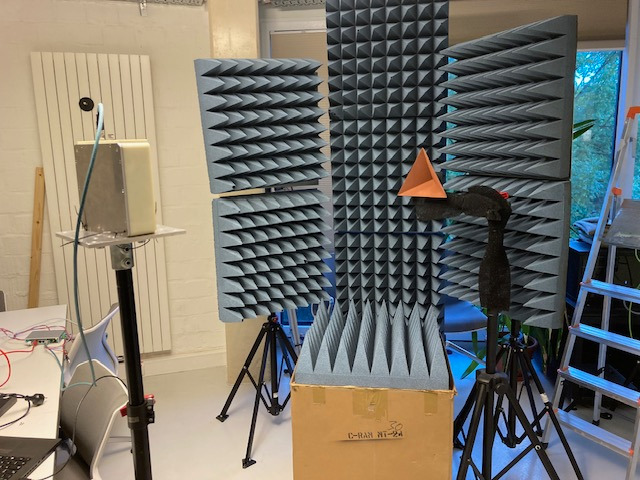
\includegraphics[height=0.25\textheight]{../figures/aufbau1.jpg}
    \caption{Measurement Setup}
    \label{fig:photo_setup}
\end{figure}
\begin{figure}
    \centering
    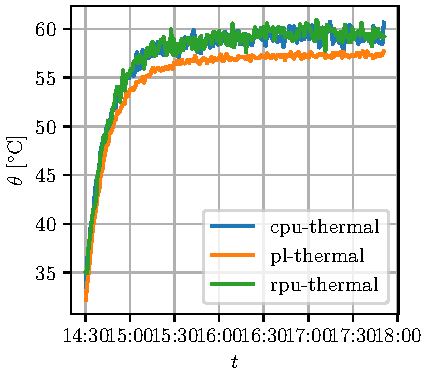
\includegraphics[height=0.25\textheight]{../figures/actual_temperature.pdf}
    \caption{Measured System Temperature After Startup}
    \label{fig:act_temp}
\end{figure}

Due to the geometry of the setup, the runtime of each transmitted wavefront should be identical.
Thus, the ideal deramped signal should be of a single, constant frequency and without inter-channel phase differences.
\begin{figure}
    \centering
    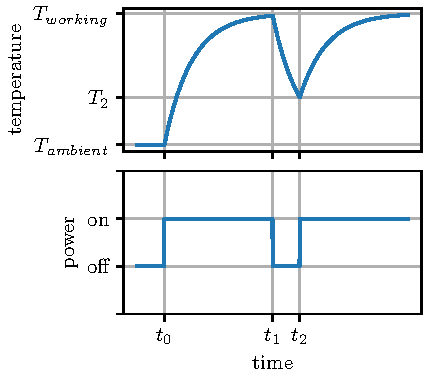
\includegraphics[height=0.25\textheight]{../figures/expected_temperature.pdf}
    \caption{Expected System Temperature over Time for Interrupted Power}
    \label{fig:exp_temp}
\end{figure}
In practice, the reflector peak will have a certain bandwidth,
and other peaks at higher and lower frequencies will be present due to incomplete shielding and/or unwanted reflections.
Also, the reflector peak may wander if the setup geometry moves. \\
For analysis, system runtime and temperature cannot be considered independent variables, as illustrated in figure \ref{fig:exp_temp}:
The system starts at ambient temperature, heating up and approaching a stable operating temperature on turning on ($t_0$), and cooling back down after turning off ($t_1$). \\
\begin{figure}[h]
    \centering
    \begin{subfigure}[t]{.45\textwidth}
        \centering
        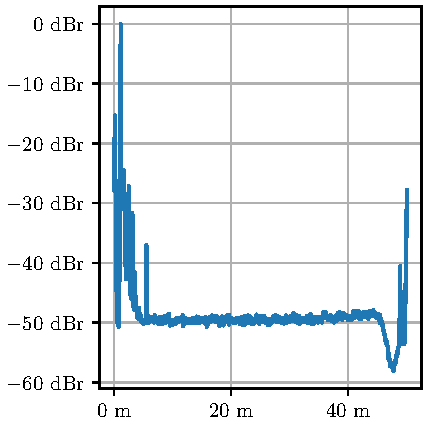
\includegraphics[width=\textwidth]{../figures/interference.pdf}
        \caption{Complete Spectrum}
    \end{subfigure}
    \begin{subfigure}[t]{.45\textwidth}
        \centering
        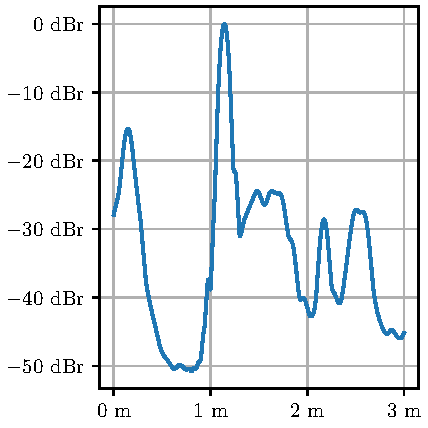
\includegraphics[width=\textwidth]{../figures/interference_zoom.pdf}
        \caption{Zoomed in}
    \end{subfigure}
    \caption{Mean Intensity Spectrum}
    \label{fig:avg_intensity}
\end{figure}
\subsection{Preprocessing and Analysis}
Because of the aforementioned imperfections in the experiment, some preprocessing is required to analize the systematic offsets present in the radar signal.
Multiple additional peaks in the spectrum are visible in figure \ref{fig:avg_intensity}; indeed, the maximum peak is not even caused by the reflector.
It is therefore necessary to limit the analysis to only the FFT-bin at the maximum of the peak caused by the reflector.

The measurement environment also exhibits some minor changes in temperature and humidity, which can result in the geometry to shift by a few millimeters.
This shows by the spectral maximum shifting over time, as seen in figure \ref{fig:refldist}.

\begin{figure}
    \centering
    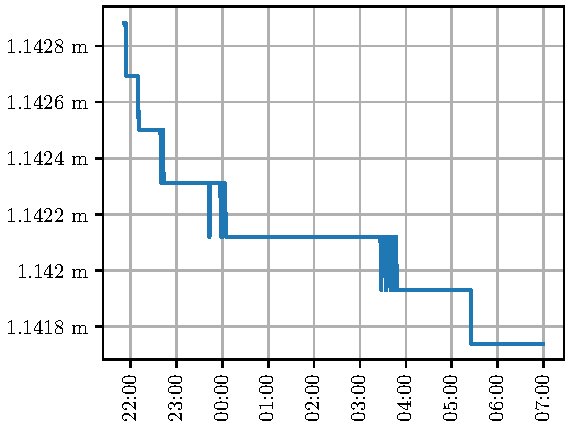
\includegraphics[width=\textwidth]{../figures/refldist.pdf}
    \caption{Change in reflector distance as measured by iMCR}
    \label{fig:refldist}
\end{figure}

In the following analysis, the main metric is the complex ratio of the maximum FFT-bin to its initial value.
Using a logarithmic representation  of this ratio, it can be represented as a level difference [\unit{\decibel}] and a phase difference [\unit{\degree}].

\subsection{Effects of System Temperature and Runtime}

Multiple measurements have indicated that, while the amplitude rarely varies by more than \SI{1}{\decibel}, the phase is not as stable over time.
Typically, the mean phase drifts by up to \SI{50}{\degree} in the hours after system startup, with the rate of change reducing after around four hours.
However, it has to be noted that there is no clear correlation between phase drift and temperature:
the phase continues to drift after the system temperature stabilizes;
the reduction in drift only occurs hours after the system has reached a stable temperature of approximately \SI{60}{\celsius}.

\begin{figure}
    \centering
    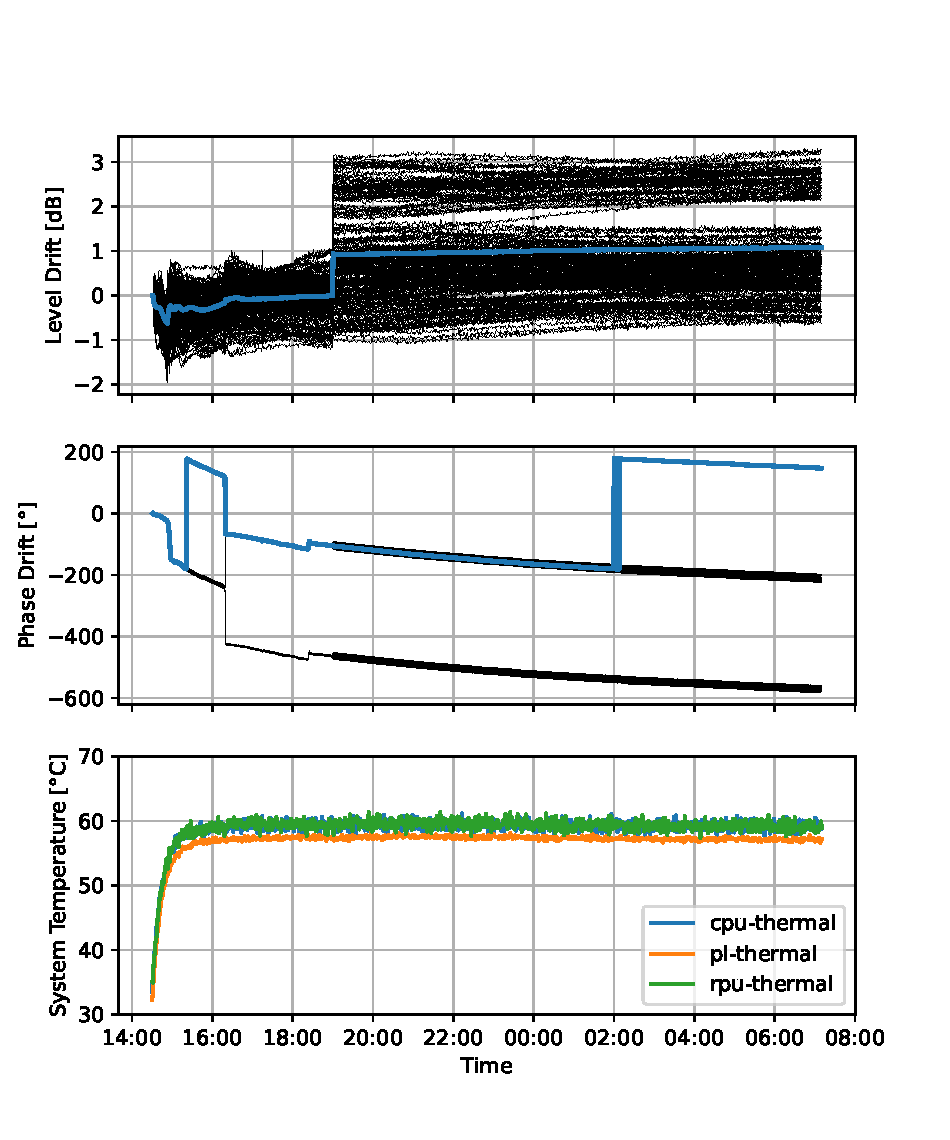
\includegraphics[width=\textwidth]{../figures/meas_23-10-09_phase_drift.pdf}
    \caption{Recorded drift over night}
    \label{fig:weekend}
\end{figure}
TODO : split new measurement into heating up (23:00-8:00) and stable (13:00-12:00).


\subsection{Effects of Self-Calibration}
As described in the specification, the AWR2243P-chips undergo a self-calibration upon initialization.
This initialization can be triggered by either restarting the entire system or by re-writing the configuration registers on the radar chips.
Indeed, this initial calibration can be observed in the data (cf. \ref{fig:restart}).
After the connection with the radar has been re-established, the following effects are visible:
\begin{itemize}
    \item slightly increased level: the level in each channel increases by approximately \SI{0.3}{\decibel}
    \item increased incoherence: after the first restart of the system, the drift in both level and phase is distributed more broadly
    \item mean phase: the mean phase drift changes by up to \SI{5}{\degree}
\end{itemize}

\begin{figure}
    \centering
    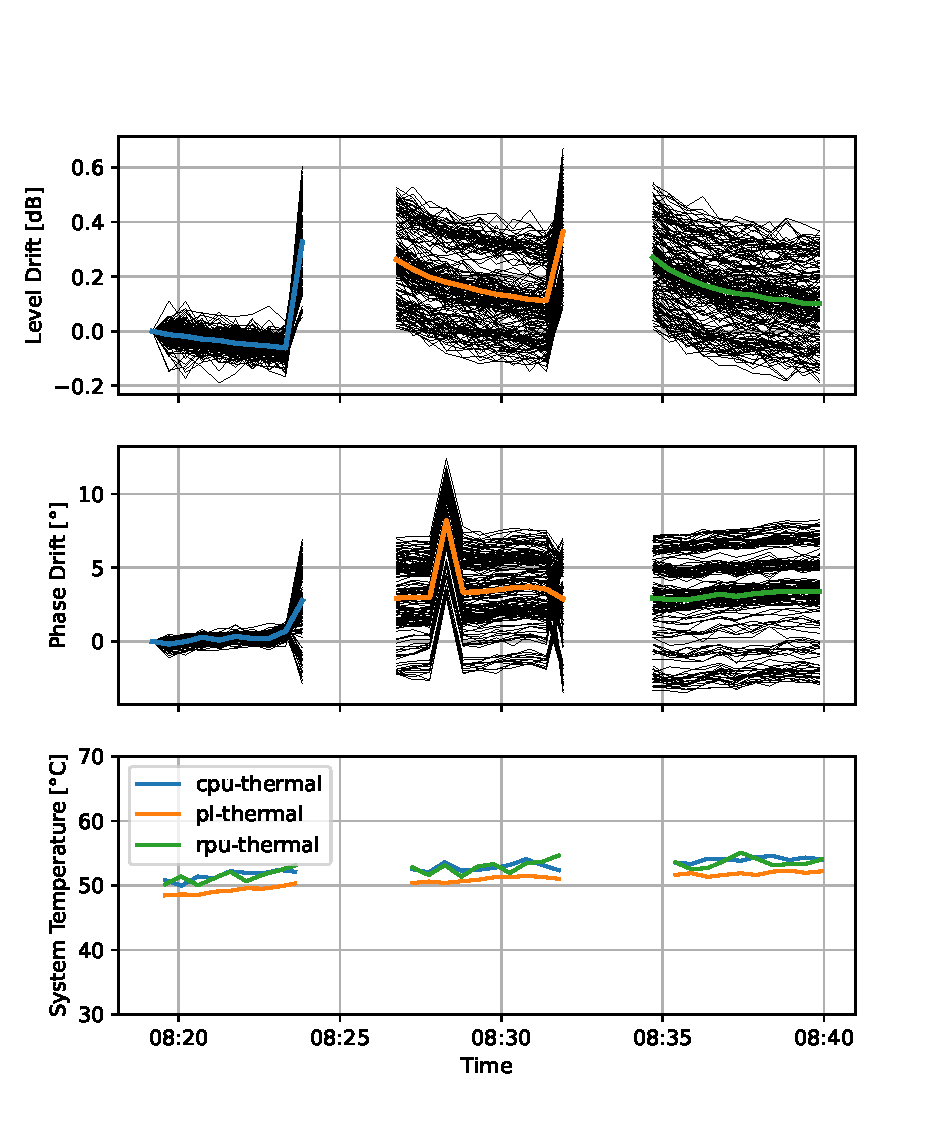
\includegraphics[width=\textwidth]{../figures/meas_23-10-30_reboots_phase_drift.pdf}
    \caption{Recorded drift and temperature with system restart}
    \label{fig:restart}
\end{figure}

TODO: graph jumps to new phase before reboot. confirm or fix.

TODO: quantify amount of discontinuity


\subsection{Antenna Separation}
TODO: split gains like in 3.3.7

\subsection{Differences between Antennas}
TODO: Plots, antenna Separation

Comparing the amplitude recorded by all antenna pairs, no channel in particular stands out [PLOT NEEDED].
When looking at the different channels phase drifts, it can be seen that the array becomes less coherent over time.
The distribution of phase shift across channels seems roughly gaussian [PLOT NEEDED], with increasing variance over time.
No antenna pair seems more prone to incoherence than the rest:
across measurements, the maximum outlier (in terms of divergence from the mean phase) cannot be associated with a chip or antenna.

\subsection{Conclusion}
The systematic offsets of the system are now better described.
While the amplitude of the measured signal is relatively stable, the phase is affected more strongly.
All channels' phases drift from both their initial value and each other over time.
It can also be demonstrated that restarting the radar frontend has an effect on the phase, since the frontend undergoes an automatic calibration each time.
No clear bias within the array has been found, seeing that across multiple measurements, all channels seem to be affected similarly.

Overall, it has been demonstrated that the radar system cannot be considered ideal and
its imaging fidelity will be affected by the growing incoherence during long runtimes.
Furthermore, restarting the system will change the systematic offsets due to the automatic calibration of the radar frontend hardware.
Adaptive online calibration would be required to deal with these effects. \\

To limit the scope of this thesis, the focus is set on the offline-part of the calibration process.
Because the phase and amplitude offsets are affected by the automatic calibration of the system,
this calibration should ideally be repeated on every startup, ideally letting the system temperature stabilize.

An advantage for the offline calibration is that the speed at which the array incoherence grows is limited.
That means that for sufficiently short runtimes, it can be assumed to be static, and therefor, an offline calibration to be sufficient.